\chapter{Optimizations of emulated e1000 performance}
In the chapter \ref{chap:env} we have given an overview of the software environment involved in this work.
In this chapter we will analyze problems and bottlenecks of the current system implementation and propose solutions that are able
to remove them.

\vspace{0.5cm}

First of all we have to point out what we are going to optimize. We consider two scenarios.

In the first scenario, \emph{guest to guest} (G2G), two VM are run on the same host and are connected through a host-only virtual LAN (see 
section \ref{sec:qemunet}). One of the two VMs runs an application that sends UDP packets of a given size at a given average rate, while 
the other VM tries to receive all the UDP packets it can.

The second scenario, \emph{guest to host} (G2H), is similar to the first, but only a VM is present, and it runs the UDP sender application. The UDP receiver application
is run by the host.

In our experiments, we will try to give to each guest one or two VCPU, and discuss the differences between the two cases.

\begin{figure}[bt]
\centering
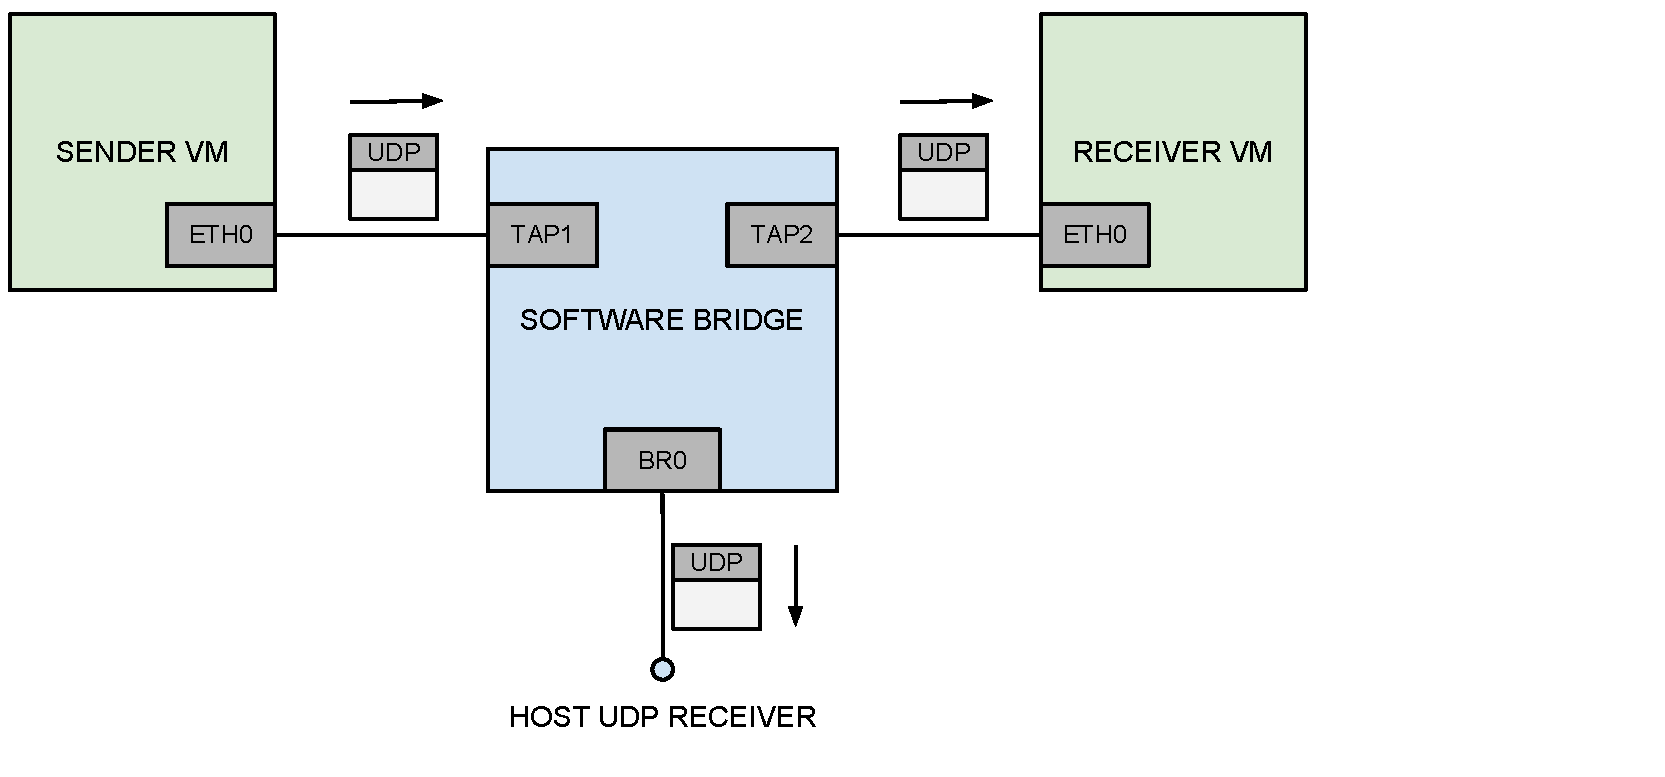
\includegraphics[scale = 0.60]{scenario.pdf}
\caption{Communication scenario in which and UDP sender is on a VM and an UDP receiver is on the host or on another VM.}
\label{fig:scenario}
\end{figure}

\vspace{0.5cm}

In these situations we want to maximize the packet rate, both on the transmit and receive side.


\section{Analysys of the existing implementation}
\label{sec:e1000perf}
We are now going to show and discuss the performance of the existing solution, e.g. of the machanisms illustrated in section 
\ref{sec:e1000emu} and \ref{sec:e1000driver}.
All the measurements have been done on a laptop machine with an i5-2450M processor, which is endowed with four cores running at 2.5GHz
\footnote{The linux CPU frequency manager has been used to set the CPU frequency at the maximum possible frequency.}.

\subsection{TX performance}
\label{sec:e1000txperf}
In this experiment a VM runs an UDP sender that sends UDP packets to an UDP receiver that runs on the host. The sender is just an 
infinite loop where each iteration invokes the \texttt{send} system call. The buffer passed to the system call is always the same and its
length is such that a minimum size ethernet frame (60 bytes) is sent on the wire for each \texttt{send}.
With this test we push to the limit the TX performances in the short packet case.


\subsubsection{1 VCPU test}
\label{sec:e1000-tx-g2h1vcpu}
The measurement results are shown in the table \ref{tab:e1000-tx-g2h1vcpu}. The guest has been assigned 1 VCPU, and all the values are computed
counting the number of occurrencies of each event over a 1 second period and then dividing the count by the period itself.

\begin{table}
\begin{center}
\begin{tabular}{lrl}
\toprule
\textbf{Interrupt rate} & 20.567 & KHz\\
\textbf{TX packet rate} & 20.567 & Kpps\\
\textbf{TX bitrate} & 14.973 & Mbps\\
\textbf{TX notifications rate} & 20.567 & KHz\\
\textbf{MMIO write rate} & 61.702 & KHz\\
\textbf{MMIO read rate} & 61.702 & KHz\\
\bottomrule
\end{tabular}
\end{center}
\caption{Guest to host statistics with 1 VCPU per guest}
\label{tab:e1000-tx-g2h1vcpu}
\end{table}

As we can see, the TX rate is very modest, about 20.5 Kpps. There is a TX notification (a write to the TDT register) and a TX interrupt for 
each packet sent. The total number of MMIO accesses is 6 times the number of interrupts.

The high MMIO access rate is due to the interrupt routine. 
When invoked, in fact, the interrupt routine has to VMExits at least 5 times:
\begin{enumerate}
    \item Reads the ICR (Interrupt Cause Read) register, in order to get the Interrupt reason (if any).
    \item Writes to the IMC (Interrupt Mask Clear) register, in order to disable the interrupts.
    \item Reads from the STATUS regsiter, in order to flush the previous register write.
    \item After the NAPI work is completed, it write to the IMS (Interrupt Mask Set) register in order to reenable the interrupts.
    \item Reads form the STATUS register, in order to flush the previous register write.
\end{enumerate}

The sixth MMIO access per interrupt is due to the TX notification.

Even if the hardware interrupt moderation is not emulated, the Linux e1000 driver uses the NAPI interface (section \ref{sec:napi}), so 
a software interrupt
moderation is actually implemented. Unfortunately, it doesn't work for TX interrupts, and the reason for this is actually very simple.
In section \ref{sec:e1000txemu} we have seen that the TX emulation is done in a synchronous way, that is the VCPU thread that writes
the to TDT register, after the VMExit, executes the e1000 frontend, the TAP backend and raises the interrupt pin. After that
it does a VMEnter coming back to the guest world, but with a TX interrupt to handle. Since the guest
has only a VCPU, the VCPU must be used to handle the interrupt, and cannot be used to insert more TX frames into the ring (e.g. to call
the \texttt{ndo\_start\_xmit} method). Consequently, the NAPI polling function will only clean the TX descriptor(s) associated to the
frame sent.
In conclusion, if we write to the TDT register every time the \texttt{ndo\_start\_xmit} method is invoked, we are doomed to receive
an interrupt for each frame we send, and so to have low performances.


\subsubsection{2 VCPUs test}
The same experiment has been done assigning 2 VCPU to the guest. The measurement results are shown in the table \ref{tab:e1000-tx-g2h2vcpu}.

\begin{table}
\begin{center}
\begin{tabular}{lrl}
\toprule
\textbf{Interrupt rate} & 23.577 & KHz\\
\textbf{TX packet rate} & 30.400 & Kpps\\
\textbf{TX bitrate} & 22.131 & Mbps\\
\textbf{TX notifications rate} & 30.400 & KHz\\
\textbf{MMIO write rate} & 61.916 & KHz\\
\textbf{MMIO read rate} & 47.274 & KHz\\
\bottomrule
\end{tabular}
\end{center}
\caption{Guest to host statistics with 2 VCPU per guest}
\label{tab:e1000-tx-g2h2vcpu}
\end{table}

Compared with the 1-VCPU case, the situation is slightly better, but still modest. Here we have about 30 Kpps, and an interrupt rate
that is significantly less than that. This means that every TX interrupt, on average, handles more than one frame.
Note that there is still only one TX frame sent for each TX notification, like in the 1-VCPU case.
The improvement is due to the higher degree of parallelism in the guest, that allows the NAPI to coalesce some interrupts, so that
on average about 1.29 data TX descriptors are cleaned for each interrupt. THis happens because while one VCPU is executing the interrupt
routine (or the NAPI context is active) with the e1000 interrupts disabled, the other VCPU can find the time to insert another TX frame
in the ring, execute the frontend and backend and return to the guest without raising an interrupt because they are disabled.
In this way sometimes the NAPI polling routines cleans more than one data TX descriptor.


\subsubsection{Discussion}
\label{sec:e1000txperfdiscuss}
The low performance is basically due to two problems: The hardware interrupt moderation is not emulated in QEMU and there is a TX 
notification for each frame to send. This is true in both 1-VPCU and 2-VCPU cases.

If we coalesced the interrupts, we could amortize the 5 VMExits and the interrupt overhead over more TX frames.
Implementing the emulation of the hardware interrupt is then then an optimization we can implement.

If we had a way to coalesce the TX notifications we could amortize the cost of a notification over more TX frames. This
a second optimization we can implement.

\vspace{0.5cm}

We've not discussed the performances with bigger packet sizes, because the problems involved are exactly the same. When the packets are 
big there is more work to do because the packet copies are more expensive, and so the performance are lower. However, we will show that
the optimization are very affective also for the big packet case, because the overhead due to the copies is significantly lower than
the overheads due to TX notifications and interrupts.



\subsection{RX performance}
In this experiment a VM runs an UDP receiver that receives UDP packets from an UDP sender that runs on the host. The receiver is just an 
infinite loop where each iteration invokes the \texttt{recvmsg} system call. No processing is made on the received packet.
The UDP sender is similar to the sender used in section \ref{sec:e1000txperf}, but after each \texttt{send} system call the process
does some busy waiting in order to send UDP packets at a given rate.
With this test we push to the limit the guest RX performances in the short packet case.

\vspace{0.5cm}

The receiving process is generally more problematic than the transmit process, because of the \emph{livelock} problem.
Wehn the incoming packet rate and/or the interrupt rate are too high, or the traffic is very irregular (e.g. it's very bursty), the guest
OS does a lot of processing (device driver and network stack) before trying to put the packet in a socket receive queue, but in the end it
is forced to throw it away because the queue is full. In its turn, the queue is full because the receiver process doesn't have enough
time to read all the packets from the queue.

For this reason there is a \emph{critical} RX packet rate that, if exceeded, causes some percentage of packets to be dropped.


\subsubsection{1 VCPU test}
\label{sec:e1000-rx-g2h1vcpu}
In this test one VPCU is assigned to the guest. The measured critical RX packet rate is about 14.4 Kpps.
This means that if the incoming packet rate is smaller that, the receiver process is able to receive very packet, and nothing is dropped.
The measurement results shown in table \ref{tab:e1000-rx-g2h1vcpu} are taken when the received rate is about the same as the critical
rate.

\begin{table}
\begin{center}
\begin{tabular}{lrl}
\toprule
\textbf{Interrupt rate} & 14.314 & KHz\\
\textbf{RX packet rate} & 14.403 & Kpps\\
\textbf{RX bitrate} & 10.485 & Mbps\\
\textbf{RX notifications} & 14.288 & Mbps\\
\textbf{MMIO write rate} & 42.861 & KHz\\
\textbf{MMIO read rate} & 42.860 & KHz\\
\bottomrule
\end{tabular}
\end{center}
\caption[H2G with 1VCPU per guest]{Host to guest statistics with 1 VCPU per guest}
\label{tab:e1000-rx-g2h1vcpu}
\end{table}

The critical RX rate is very low. If we keep incrementing the incoming RX rate beyond the critical point, the system enters a livelock 
state. Since more RX interrupt work is requested and we only have a VCPU, the receiver user process has less CPU time than before, even
if there are more packets to receive. As a result, the RX throughput seen by the user process drops immediately after the critical rate,
the system become extremely instable, and most of the packets are dropped. With packet rates higher than 15 Kpps the system becomes
inusable.

\vspace{0.5cm}

Let's analyze what happens when the livelock doesn't shows up (table \ref{tab:e1000-rx-g2h1vcpu})
The interrupt rate is a little lower than the RX packet rate, and this means that some interrupts have been coalesced by the NAPI.
This is possible even with a single VCPU, differently from what happens int the TX case, because (see section \ref{sec:e1000rxemu})
the hardware emulation (backedn and frontend) is done by the IOThread, while the guest is executed by a VCPU thread. Parallelism is 
therefore possible, because the IOThread could insert a new frame in the RX ring while the NAPI is polling, and/or the interrupt could
be delayed because the interrupts are disabled.

However, the two rates are almost the same, and so we still have approximately an interrupt for each frame received, which means that
the NAPI software moderation isn't not working well. More precisely, we have measured the distribution of the amount of RX NAPI work
done each time the polling function is called and reported it in table \ref{tab:e1000-rx-napi-dist}.

\begin{table}
\begin{center}
\begin{tabular}{lrl}
\toprule
\textbf{NAPI RX work} & \textbf{Percentage}\\
\midrule
0 & 0.05\%\\
1 & 99.485\%\\
2 & 0.335\%\\
$\geq$ 3 & 0.13\%\\
\bottomrule
\end{tabular}
\end{center}
\caption{Host to guest NAPI distribution with 1 VCPU per guest. The NAPI work is the number of
frames handled by the execution of the polling function.}
\label{tab:e1000-rx-napi-dist}
\end{table}

Why is the NAPI working so bad? The problem here isn't related to lack of parallelism, like in the TX case, but is due to the guest being
too fast. In fact, we can observe that in this experiment the overall system is composed of a \emph{producer} thread, e.g. the IOTHread,
and a \emph{consumer} thread, e.g. the VCPU thread. The producer is basically an infinite loop that on each iteration gets a frame from the
TAP, inserts it in the RX ring and raises an interrupt if enabled. The consumer is woken up by an interrupt and schedules the NAPI context.
The NAPI polling functions is a loop that on each iteration extracts an RX frame from the ring and push it to the stack, until there is no
work left.

If the consumer iteration is on average slower than the producer iteration, the latter is very likely to find the interrupts disabled
after inserting a new RX frame, and the producer is very likely to see the new frame while is executing the polling function corresponding
to a previous interrupt. In this scenario the consumer will (almost) always find work to do, and so the interrupt will (almost) always
be disabled, and consequently the NAPI mitigation will work.

On the other hand, if the consumer iteration is on average faster than the producer iteration, the latter is very likely to find the
interrupt enabled after inserting a new RX frame, and so an interrupt is raised for each received frame. This is exactly what happens
in our experiment. It's important to point out that when there is no more work to do, the NAPI polling function is forced to complete 
and reenable the interrupts, because we don't know when the next RX frame is going to come.

It's important to obeser that in this experiment the consumer is very slow simply because we have forced the UDP sender to send to a 
constant packet rate of 14 Kpps, which makes it slow by definition. We cannot go beyond 14Kpps because of the livelock.

\vspace{0.5cm}

Moreover, as we can see in the table \ref{tab:e1000-rx-g2h1vcpu}, we also have approximately a write to the RDT register (RX 
notification) for each interrupt, which is not good. This is also a consequence of the NAPI misbehaving.

Similarly to the 1-VCPU TX case, here we have 6 MMIO accesses for each interrupt. Five of them are exactly the same listed in
section \ref{sec:e1000-tx-g2h1vcpu}, while the sixth one correspond to the RX notification.


\subsubsection{2 VCPUs test}
The same experiment has been done assigning 2 VCPU to the guest. Here the critical rate is way higher, about 175 Kpps. Moreover,
if the rate is passed, the system still works, even if packets start to be dropped and it becomes unstable (the dropping percentage
varies very much between 5\% and 85\%). The performances don't drop immediately after the critical rate, like in the 1-VCPU case: The system
is still usable (but not stable) if the incoming RX rate is about 300K.

The measurement results are shown in the table \ref{tab:e1000-rx-g2h2vcpu} when the incoming packet rate is about 185 Kpps.

\begin{table}
\begin{center}
\begin{tabular}{lrl}
\toprule
\textbf{Interrupt rate} & 6.696 & KHz\\
\textbf{RX packet rate} & 185.657 & Kpps\\
\textbf{RX bitrate} & 135.158 & Mbps\\
\textbf{RX notifications} & 13.725 & Mbps\\
\textbf{MMIO write rate} & 22.661 & KHz\\
\textbf{MMIO read rate} & 13.459 & KHz\\
\bottomrule
\end{tabular}
\end{center}
\caption[H2G with 2VCPU per guest]{Host to guest statistics with 2 VCPU per guest}
\label{tab:e1000-rx-g2h2vcpu}
\end{table}

As we can see, here the NAPI works very well, since the producer here is way faster than 14 Kpps (see section \ref{sec:e1000-rx-g2h1vcpu}).
On average we serve about 27 RX frames per interrupt, so that the high interrupt overhead and the MMIO accesses are amortized.

The RX notification rate is about twice as the interrupt rate, because when the polling function handles more frames, it gives new memory
buffers to the hardware doing a write to the RDT register every 16 frames handled (see section \ref{sec:rxdriver}) and a write at the end
of the polling function. Since on average 27 frames are served, we have 2 RDT writes.


\subsubsection{Discussion}
The low performance in the 1-VCPU case is basically due to two problems: The hardware interrupt moderation is not emulated in QEMU and
there is a RX notification for each frame to send. The interrupt moderation here is necessary, because the NAPI mitigation doesn't work
(because of the livelock).

In the 2-VCPU case the mitigation can still be useful to remove the existing fluctuations in the interrupt rate which cause performance
drops, and in general the system to be more stable. In our experiment, in fact, we noted that the performance drops when the interrupt
rate has a peak (~10 KHz).

The second problem has minor negative effects on performance in the 2-VPCU case, because at least an RX notification is done every
16 frames.

\vspace{0.5cm}

We've not discussed the performances with bigger packet sizes, for the same reasons explained in \ref{sec:e1000txperfdiscuss}.



\section{Implementing interrupt moderation}
In section \ref{sec:e1000txperf} we have seen that we can improve both the RX and TX packet rate if we emulate the e1000 mitigation.
A precise emulation is not necessary nor possible, and it's therefore convenient to choose a simple and efficient one.
In this work we decide to implement the ITR register, the TADV register and the RADV register.
We are not interested in the TIDV and RDTR register\footnote{However, the RDTR register has been added to the frontend only to 
validate the RADV content. The e1000 speicification, in fact, says that the TADV register is not valid if RDTR contains 0.}.

\vspace{0.5cm}

In our implementation we use a single QEMUTimer (see section \ref{sec:qemuel}, even if the hardware has multiple timers, so we have to 
aggregate the meaning o the ITR, TADV and RADV registers.
We therefore consider the moderation delay to be the minimum delay among the ones specified through the ITR, TADV and RADV registers.
When computing the minimum, each register is considered only if the content is valid and if there is a proper event type pending.
According to the e1000 specification a zero value means that the register content is not valid. If there is no pending TX event
the TADV content is not considered, while if there is no pending RX event the RADV register is not considered.

Moreover, only the interrupts due to transmission (\texttt{start\_xmit} function) and reception (\texttt{e1000\_receive}
function) are considered. The other interrupts are extremely rare, so they are not intersting.


\vspace{0.5cm}
Let's see how moderation is implemented. We have modified the code so that the frontend calls the \texttt{mit\_set\_ics} function instead
of the \texttt{set\_ics} function when it wantsto issue an interrupt.
The first time is called, the \texttt{mit\_set\_ics} arms the moderation timer (\texttt{mit\_timer}) with the moderation delay and issues 
an interrupt.
When the function is called again, if the timer has not expired yet, it only accumulates the interrupt cause, but don't issue an interrupt.
When the timer expires, an interrupt is sent, and the timer is rearmed only if there is a pending accumulated interrupt cause and
the moderation delay is not zero.
Every time the timer is (re)armed the moderation delay is computed again, because the mitigation registers content can change, and
the pending events could be only RX or only TX events.

In this way we are sure that the minimum inter-interrupt interval is always greater or equal than the moderation delay.

\vspace{0.5cm}

The proposed moderation patch adds about 50 lines of code to the e1000 frontend (hw/e1000.c).



\subsection{Improvements analysys}
In this section we will repeat the same experiments presented in section \ref{sec:e1000perf} in order to see the improvements obtained
with the the moderation patch. With this experiment the Linux e1000 module has been loaded specifying the following parameters:
\begin{center}
\begin{tabular}{ll}
\toprule
\textbf{Parameter} & \textbf{Value}\\
\midrule
TxIntDelay & 0\\
TxAbsIntDelay & 0\\
InterruptThrottleRate & 4000\\
\bottomrule
\end{tabular}
\end{center}

In this way we only use the new moderation mechanism (e.g. ITR). It's not necessary to specify the parameters relative to RDTR and
RADV, since RDTR is 0 by default (so both RDTR and RADV are disabled). The InterruptThrottleRate parameter actually specifies the Maximum
Allowed Interrupt Rate (MAIR), which is inversely proportional to the value that the driver has to put in the ITR register in order to limit
the interrupt rate.

\subsection{TX performance}
\label{sec:e100-mit-tx}
The results n the 1-VCPU case is shown in table \ref{tab:e1000-mit-tx-g2h1vcpu}.

\begin{table}
\begin{center}
\begin{tabular}{lrl}
\toprule
\textbf{Interrupt rate} & 3.805 & KHz\\
\textbf{TX packet rate} & 47.849 & Kpps\\
\textbf{TX bitrate} & 34.834 & Mbps\\
\textbf{TX notifications rate} & 47.849 & KHz\\
\textbf{MMIO write rate} & 55.464 & KHz\\
\textbf{MMIO read rate} & 11.478 & KHz\\
\bottomrule
\end{tabular}
\end{center}
\caption{Guest to host statistics with 1 VCPU per guest when interrupt moderation is implemented.}
\label{tab:e1000-mit-tx-g2h1vcpu}
\end{table}

As we can see from the table, there is an important improvement. The interrupt rate is less than 4 KHz, and this is what we expected to see
since we have set the MAIR to 4000.
With reference to the existing implementation (section \ref{sec:e1000-tx-g2h1vcpu}, we have a performance gain of 2.32, with about 47 Kpps.
Since the interrupts are coalesced by the interrupt moderation mechanism, the NAPI polling function cleans on average 12.58 TX data 
descriptors each time is called. Remember that the TX emulation is synchronous with the guest VPCU (see section\ref{sec:e1000txperf}), and
so the NAPI software moderation it's useless by itself.

Despite of the good improvements, we still have a TX notification for each frame sent, and the performances are greatly limited by this
problem.

\vspace{0.5cm}

In order to understand the mitigation effects on performances, we have tried different MAIR values, computing the average TX packet 
rate on a very long time window (some minutes). The results are shown in figure \ref{fig:itr-vs-txrate}.
From this plot we can see that the lower the MAIR is, the higher the TX packet rate is. However we cannot set MAIR to a value too low,
because this would increment the latency too much. In fact while the moderation timer is on, we don't let the emulated hardware raise
any interrupt, and so the responsivity is limited by the moderation delay, namely by the ITR.
As stated previously, in this study we want to maximize the packet rate, and we are not interested in minimizing the latency.

\begin{figure}[bt]
\centering
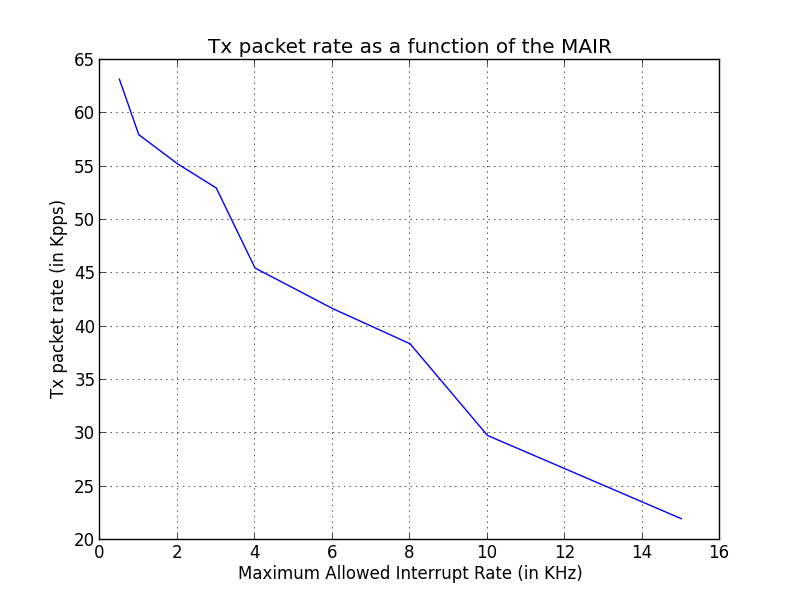
\includegraphics[scale = 0.7]{MAIR-vs-TXRate.png}
\caption{Measured TX rate as a function of the Maximum Allowed Interrupt Rate.}
\label{fig:itr-vs-txrate}
\end{figure}

\vspace{0.5cm}

The measured results in the 2-VCPU case are shown in table \ref{tab:e1000-mit-tx-g2h2vcpu}.

\begin{table}
\begin{center}
\begin{tabular}{lrl}
\toprule
\textbf{Interrupt rate} & 3.806 & KHz\\
\textbf{TX packet rate} & 47.169 & Kpps\\
\textbf{TX bitrate} & 34.339 & Mbps\\
\textbf{TX notifications rate} & 47.169 & KHz\\
\textbf{MMIO write rate} & 54.778 & KHz\\
\textbf{MMIO read rate} & 11.469 & KHz\\
\bottomrule
\end{tabular}
\end{center}
\caption{Guest to host statistics with 2 VCPU per guest when interrupt moderation is implemented.}
\label{tab:e1000-mit-tx-g2h2vcpu}
\end{table}

The results are similar to the 1-VCPU case, because the incremented parallelism is not exploited. Even if there is parallelism
between the interrupt routine and the transmission path, the TX clean work is not very expensive. Therefore we don't benefit from a second 
VCPU, or the little benefits are compensated by the overhead involved in the SMP management (e.g. locks).


\subsection{RX performance}
The measured critical rate with 1-VCPU is about 150 Kpps.
The table \ref{tab:e1000-mit-rx-g2h1vcpu} shows the results obtained when the incoming RX rate is about 137 Kpps.

\begin{table}
\begin{center}
\begin{tabular}{lrl}
\toprule
\textbf{Interrupt rate} & 3.838 & KHz\\
\textbf{RX packet rate} & 137.103 & Kpps\\
\textbf{RX bitrate} & 99.811 & Mbps\\
\textbf{RX notifications} & 10.322 & Mbps\\
\textbf{MMIO write rate} & 17.990 & KHz\\
\textbf{MMIO read rate} & 11.502 & KHz\\
\bottomrule
\end{tabular}
\end{center}
\caption{Host to guest statistics with 1 VCPU per guest, when interrupt moderation is implemented.}
\label{tab:e1000-mit-rx-g2h1vcpu}
\end{table}

As we can see, there is a huge improvement in the packet rate performance, because on average we amortize the interrupt related overhead
over about 35 frames. Since the interrupt rate is lower, also the RX notification rate is lower. On average we should expect 
$\lfloor \frac{35}{16} \rfloor + 1 = 3$ RDT writes for each interrupt (see section \ref{sec:rxdriver}), and so a notification rate of 
about $3 \cdot 3.838 KHz = 11.514 KHz$, which is similar to the measured one (10.332 KHz).

If we increase the incoming RX rate, the performance of the UDP receiver gradually degrades, but we don't incur in a complete livelock 
(like the livelock we have seen in section \ref{sec:e1000-rx-g2h1vcpu}), because the interrupt rate is bounded.

\vspace{0.5cm}

In order to understand the mitigation effects on performances, we have tried different MAIR values, measuring the critical rate for
each value. The measurements are shown in figure \ref{fig:itr-vs-cr}.
The plot shows that if we increase the MAIR in in the region [2 KHz, $+\infty$], the performances gradually decrease, since we are 
less and less restrictive on the Maximum Allowed Interrupt Rate.
On the other end, if we decrease the MAIR below 1.5 KHz, the throughput starts to decrease, because the RX ring gets full and the guest
is not notified in a timely manner.
Moreover, we cannot choose the MAIR to be too low because of the latency (see section \ref{sec:e100-mit-tx});

\begin{figure}[bt]
\centering
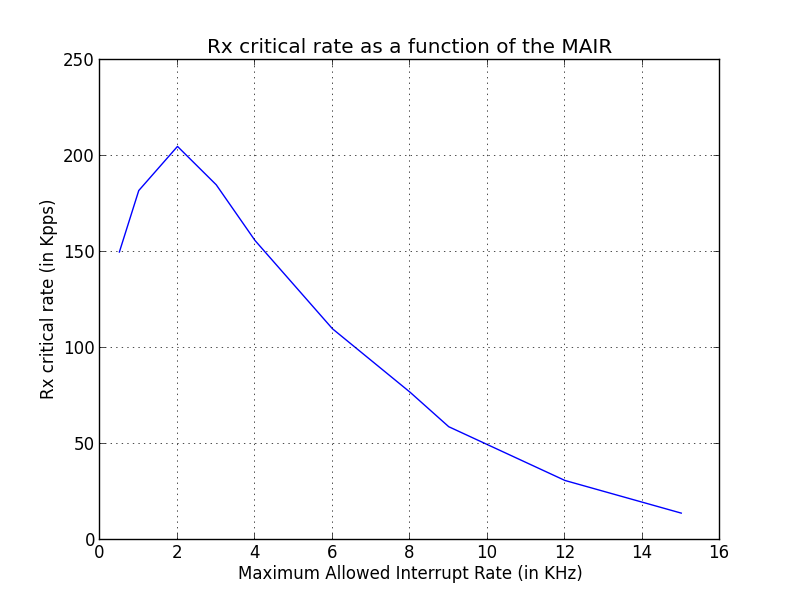
\includegraphics[scale = 0.7]{MAIR-vs-CR.png}
\caption{Measured critical rate as a function of the maximum allowed Interrupt Rate.}
\label{fig:itr-vs-cr}
\end{figure}


\vspace{0.5cm}

The 2-VCPU case results (MAIR = 4 KHz, incoming RX rate = 240 Kpps) are shown in table \ref{tab:e1000-mit-rx-g2h2vcpu}

\begin{table}
\begin{center}
\begin{tabular}{lrl}
\toprule
\textbf{Interrupt rate} & 2.098 & KHz\\
\textbf{RX packet rate} & 216.674 & Kpps\\
\textbf{RX bitrate} & 157.739 & Mbps\\
\textbf{RX notifications} & 14.321 & Mbps\\
\textbf{MMIO write rate} & 18.511 & KHz\\
\textbf{MMIO read rate} & 6.285 & KHz\\
\bottomrule
\end{tabular}
\end{center}
\caption{Host to guest statistics with 1 VCPU per guest, when interrupt moderation is implemented.}
\label{tab:e1000-mit-rx-g2h2vcpu}
\end{table}

Similarly to what happens without moderation, a second VCPU improves the RX performance, because the improved parallelism makes the
NAPI moderation to play an active role.
The measured critical rate is about 215 Kpps (+37\% w.r.t. 1-VCPU case).
We can see that the NAPI mitigation is effective observing that the average interrupt rate is half part of the MAIR, and so the MAIR is not
restrictive at operating speed. On average we have about 103 RX frames served for each interrput, which a very good result.
The expected average RX notification rate is $(\lfloor \frac{103}{16} \rfloor + 1) \cdot 2.098$ Khz = 14.686, which is very similar to
the measured result (14.321 KHz).